\mfpicnumber{1}

\opengraphsfile{AugMatrices}

\setcounter{footnote}{0}

\label{AugMatrices}

\setlength{\extrarowheight}{0pt}

In Section \ref{LinSystems} we introduced Gaussian Elimination as a means of transforming a system of linear equations into triangular form with the ultimate goal of producing an equivalent system of linear equations which is easier to solve.  If we take a step back and study the process, we see that all of our moves are determined entirely by the \textit{coefficients} of the variables involved, and not the variables themselves.  Much the same thing happened when we studied long division in Section \ref{Polydivision}. Just as we developed synthetic division to streamline that process, in this section, we introduce a similar bookkeeping device to help us solve systems of linear equations.  To that end, we define a \index{matrix ! definition} \textbf{matrix} as a rectangular array of real numbers.  We typically enclose matrices with square brackets, `$\left[ \right.$' and `$\left. \right]$', and we size matrices by the number of rows and columns they have.  For example, the \index{matrix ! size} \textbf{size} (sometimes called the \index{matrix ! dimension} \index{dimension ! of a matrix} \textbf{dimension}) of 

\[ \left[ \begin{array}{rrr} 3 & 0 & -1 \\ 
2 & -5 & 10 \end{array} \right]\] 

is  $2 \times 3$  because it has $2$ rows and $3$ columns.  The individual numbers in a matrix are called its \index{matrix ! entry} \index{entry ! in a matrix} \textbf{entries} and are usually labeled with double subscripts: the first tells which row the element is in and the second tells which column it is in.  The rows are numbered from top to bottom and the columns are numbered from left to right.  Matrices themselves are usually denoted by uppercase letters ($A$, $B$, $C$, etc.) while their entries are usually denoted by the corresponding letter.  So, for instance, if we have 

\[ A = \left[ \begin{array}{rrr} 3 & 0 & -1 \\ 
2 & -5 & 10 \end{array} \right]\] 

then $a_{\mbox{\tiny$11$}} = 3$, $a_{\mbox{\tiny$12$}} = 0$, $a_{\mbox{\tiny$13$}} = -1$, $a_{\mbox{\tiny$21$}} = 2$, $a_{\mbox{\tiny$22$}} = -5$, and $a_{\mbox{\tiny$23$}} = 10$.  We shall explore matrices as mathematical objects with their own algebra in Section \ref{MatArithmetic} and introduce them here solely as a bookkeeping device.  Consider the system of linear equations  from number 2 in Example \ref{GaussEqnEx}

\[\left\{ \begin{array}{lrcr} (E1) & 2x+3y-z & = & 1 \\ 
(E2) & 10x-z & = & 2 \\ 
(E3) & 4x-9y+2z & = & 5 \\ \end{array} \right.\]  

We encode this system into a matrix by assigning each equation to a corresponding row.  Within that row, each variable and the constant gets its own column, and to separate the variables on the left hand side of the equation from the constants on the right hand side, we use a vertical bar, $|$.  Note that in $E2$, since $y$ is not present, we record its coefficient as $0$. The matrix associated with this system is 

\[ \begin{array}{c} \begin{array}{rrrrrrr} & & & \hspace{.33in} x & \hspace{.12in} y & \hspace{.1in} z & \hspace{.03in} c \\ \end{array} \\  \begin{array}{r} (E1) \rightarrow \\ (E2) \rightarrow \\ (E3) \rightarrow \end{array}  \left[ \begin{array}{rrr|r} 2 & 3 & -1 & 1\\ 10 & 0 & -1 & 2 \\ 4 & -9 & 2 & 5 \end{array} \right] \end{array} \]  

This matrix is called an \index{matrix ! augmented} \index{augmented matrix} \textbf{augmented matrix} because the column containing the constants is appended to the matrix containing the coefficients.\footnote{We shall study the coefficient and constant matrices separately in Section \ref{MatArithmetic}.}  To solve this system, we can use the same kind operations on the \textit{rows} of the matrix that we performed on the \textit{equations} of the system. More specifically, we have the following analog of Theorem \ref{equationmoves} below.

\smallskip

\colorbox{ResultColor}{\bbm

\begin{thm}  \label{rowops} \textbf{Row Operations:}  Given an augmented matrix for a system of linear equations, the following row operations produce an augmented matrix which corresponds to an equivalent system of linear equations. \index{matrix ! row operations} \index{row operations for a matrix}

\begin{itemize}

\item  Interchange any two rows.

\item  Replace a row with a nonzero multiple of itself.\footnote{That is, the row obtained by multiplying each entry in the row by the same nonzero number.}

\item  Replace a row with itself plus a nonzero multiple of another row.\footnote{Where we add entries in  corresponding columns.}

\end{itemize}

\end{thm}  

\ebm}

\smallskip 

As a demonstration of the moves in Theorem \ref{rowops}, we revisit some of the steps that were used in solving the systems of linear equations in Example \ref{GaussEqnEx} of Section \ref{LinSystems}.  The reader is encouraged to perform the indicated operations on the rows of the augmented matrix to see that the machinations are identical to what is done to the coefficients of the variables in the equations. We first see a demonstration of switching two rows using the first step of part 1 in Example \ref{GaussEqnEx}. 

\[\begin{array}{ccc}

\left\{  \begin{array}{lrcr}

(E1) & 3x-y+z & = & 3 \\
(E2) & 2x-4y+3z & = & 16 \\
(E3)  &  x-y+z & = & 5 \\ 

\end{array} \right.

&
\xrightarrow{\text{Switch $E1$ and $E3$}}

&

\left\{ \begin{array}{lrcr}

(E1) & x-y+z & = & 5 \\
(E2) & 2x-4y+3z & = & 16 \\
(E3) & 3x-y+z & = & 3 \\

\end{array} \right.

\end{array}\]

\[\begin{array}{ccc}

\left[ \begin{array}{rrr|r} 
3 & -1 & \hphantom{-}1 & 3 \\ 
2 & -4 & 3 & 16 \\ 
1 & -1 & 1 & 5  \\
\end{array} \right]

&
\xrightarrow{\text{Switch $R1$ and $R3$}}

&

\left[ \begin{array}{rrr|r} 
1 & -1 & \hphantom{-}1 & 5  \\
2 & -4 & 3 & 16 \\ 
3 & -1 & 1 & 3 \\ 

\end{array} \right]

\end{array}\]

Next, we have a demonstration of replacing a row with a nonzero multiple of itself using the first step of part 3 in Example \ref{GaussEqnEx}.

 \[\begin{array}{ccc}

\left\{ 

\begin{array}{lrcr}

(E1) & 3x_{\mbox{\tiny$1$}} +x_{\mbox{\tiny$2$}} + x_{\mbox{\tiny$4$}} & = & 6 \\   
(E2) & 2x_{\mbox{\tiny$1$}} + x_{\mbox{\tiny$2$}} -x_{\mbox{\tiny$3$}}  & = & 4  \\
(E3) &  x_{\mbox{\tiny$2$}} -3x_{\mbox{\tiny$3$}} -2x_{\mbox{\tiny$4$}} & = & 0 \\

\end{array} 

\right.

&
\xrightarrow{\text{Replace $E1$ with $\frac{1}{3}E1$}}

&

\left\{ 

\begin{array}{lrcr}

(E1) & x_{\mbox{\tiny$1$}} + \frac{1}{3}x_{\mbox{\tiny$2$}} + \frac{1}{3}x_{\mbox{\tiny$4$}} & = & 2 \\  
(E2) & 2x_{\mbox{\tiny$1$}} + x_{\mbox{\tiny$2$}} -x_{\mbox{\tiny$3$}}  & = & 4  \\
(E3) &  x_{\mbox{\tiny$2$}} -3x_{\mbox{\tiny$3$}} -2x_{\mbox{\tiny$4$}} & = & 0 \\

\end{array} 

\right.

\end{array}\]

\[\begin{array}{ccc}

\left[ \begin{array}{rrrr|r} 
3 & \hphantom{-} 1 & 0 & 1 & 6  \\
2 & 1 & -1 & 0 & 4 \\ 
0 & 1 & -3 & -2 & 0 \\ 

\end{array} \right]

&
\xrightarrow{\text{Replace $R1$ with $\frac{1}{3}R1$}}

&

\left[ \begin{array}{rrrr|r} 
1 & \frac{1}{3} & 0 & \frac{1}{3} & 2  \\
2 & \hphantom{-}1 & -1 & 0 & 4 \\ 
0 & 1 & -3 & -2 & 0 \\ 

\end{array} \right]
\end{array}\]

Finally, we have an example of replacing a row with itself plus a multiple of another row using the second step from part 2 in Example \ref{GaussEqnEx}.

\[ \begin{array}{ccc}

\left\{ 

\begin{array}{lrcr}

(E1) & x+\frac{3}{2}y-\frac{1}{2}z & = & \frac{1}{2} \\ 
(E2) & 10x-z & = & 2 \\
(E3) &  4x-9y+2z & = & 5 \\

\end{array} 

\right.
&
\xrightarrow[\text{Replace $E3$ with $-4E1 + E3$}]{\text{Replace $E2$ with $-10E1 + E2$}}

&

\left\{ 

\begin{array}{lrcr}

(E1) & x+\frac{3}{2}y-\frac{1}{2}z & = & \frac{1}{2} \\ 
(E2) & -15y+4z & = & -3 \\
(E3) & -15y+4z & = & 3 \\

\end{array} 

\right.
 \end{array} \]
 
\[\begin{array}{ccc}

\left[ \begin{array}{rrr|r} 
1 & \frac{3}{2} & -\frac{1}{2} & \frac{1}{2}  \\
10 & 0 & -1 & 2 \\ 
4 & -9 & 2 & 5 \\ 

\end{array} \right]

&
\xrightarrow[\text{Replace $R3$ with $-4R1 + R3$}]{\text{Replace $R2$ with $-10R1 + R2$}}
&

\left[ \begin{array}{rrr|r} 
1 & \frac{3}{2} & -\frac{1}{2} & \frac{1}{2}  \\
0 & -15 & 4 & -3 \\ 
0 & -15 & 4 & 3 \\ 

\end{array} \right]

\end{array}\]

The matrix equivalent of `triangular form' is \index{matrix ! row echelon form} \index{row echelon form} \textbf{row echelon form}.  The reader is encouraged to refer to Definition \ref{systemtriangularform} for comparison.  Note that the analog of `leading variable' of an equation is `leading entry' of a row.  Specifically, the first nonzero entry (if it exists) in a row is called the  \index{matrix ! leading entry} \textbf{leading entry} of that row.
 
\smallskip

\colorbox{ResultColor}{\bbm  

\begin{defn} \label{rowechelonform} A matrix is said to be in \textbf{row echelon form} provided all of the following conditions hold:

\begin{enumerate}

\item  The first nonzero entry in each row is $1$.

\item  The leading $1$ of a given row must be to the right of the leading $1$ of the row above it.

\item  Any row of all zeros cannot be placed above a row with nonzero entries.

\end{enumerate}



\end{defn}

\ebm}

\smallskip

To solve a system of a linear equations using an augmented matrix, we encode the system into an augmented matrix and  apply Gaussian Elimination to the rows to get the matrix into row-echelon form.  We then decode the matrix and back substitute.  The next example illustrates this nicely.

\begin{ex}  \label{GaussExMatrix} Use an augmented matrix to transform the following system of linear equations into triangular form. Solve the system.
\[\left\{ \begin{array}{rcl} 3x  - y  + z & = & 8 \\ x +  2y  -  z & = & 4 \\  2x+ 3y - 4z & = & 10 \\  \end{array} \right.\]

{\bf Solution.}  We first encode the system into an augmented matrix.

\[ \begin{array}{ccc}

\left\{ \begin{array}{rcl} 3x  - y  + z & = & 8 \\ x +  2y  -  z & = & 4 \\  2x+ 3y - 4z & = & 10 \\  \end{array} \right.

&

\xrightarrow{\text{Encode into the matrix}}

&

 \left[ \begin{array}{rrr|r} 3 & -1 & 1 & 8 \\ 1 & 2 & -1 & 4 \\ 2 & 3 & -4 & 10 \\ \end{array} \right]
 
 
 \end{array}\]

Thinking back to Gaussian Elimination at an equations level, our first order of business is to get $x$ in $E1$ with a coefficient of $1$.  At the matrix level, this means getting a leading $1$ in $R1$.  This is in accordance with the first criteria in Definition \ref{rowechelonform}.  To that end, we interchange $R1$ and $R2$.  

\[\begin{array}{ccc}

\left[ \begin{array}{rrr|r} 
3 & -1 & 1 & 8 \\ 
1 & 2 & -1 & 4 \\ 
2 & 3 & -4 & 10 \\ 
\end{array} \right]

& 

\xrightarrow{\text{Switch $R1$ and $R2$}}

&

\left[ \begin{array}{rrr|r}
1 & 2 & -1 & 4 \\  
3 & -1 & 1 & 8 \\ 
2 & 3 & -4 & 10 \\ 
\end{array} \right]


\end{array}\]



Our next step is to eliminate the $x$'s from $E2$ and $E3$.  From a matrix standpoint, this means we need $0$'s below the leading $1$ in $R1$.  This guarantees the leading $1$ in $R2$ will be to the right of the leading $1$ in $R1$ in accordance with the second requirement of Definition \ref{rowechelonform}.

\[\begin{array}{ccc}

\left[ \begin{array}{rrr|r}
1 & 2 & -1 & 4 \\  
3 & -1 & 1 & 8 \\ 
2 & 3 & -4 & 10 \\ 
\end{array} \right]
&
\xrightarrow[\text{Replace $R3$ with $-2R1+R3$}]{\text{Replace $R2$ with $-3R1 +R2$}} 
&
\left[ \begin{array}{rrr|r}  
1 & 2 & -1 & 4 \\  
0 & -7 & 4 & -4 \\ 
0 & -1 & -2  & 2 \\ 
\end{array} \right]



\end{array}\]

Now we repeat the above process for the variable $y$ which means we need to get the leading entry in $R2$ to be $1$.

\[\begin{array}{ccc}

\left[ \begin{array}{rrr|r}  
1 & 2 & -1 & 4 \\  
0 & -7 & 4 & -4 \\ 
0 & -1 & -2  & 2 \\ 
\end{array} \right]  
& 
\xrightarrow{\text{Replace $R2$ with $-\frac{1}{7}R2$}}  
& 
\left[ \begin{array}{rrr|r} 
1 & 2 & -1 & 4 \\ 
0 & 1 & -\frac{4}{7} & \frac{4}{7} \\ 
0 & -1 & -2 & 2 \\
\end{array} \right]

\end{array}\]

To guarantee the leading $1$ in $R3$ is to the right of the leading $1$ in $R2$, we get a $0$ in the second column of $R3$.

\[ \begin{array}{ccc}

\left[ \begin{array}{rrr|r} 
1 & 2 & -1 & 4 \\ 
0 & 1 & -\frac{4}{7} & \frac{4}{7} \\ 
0 & -1 & -2 & 2 \\ 
\end{array} \right]  
& 
\xrightarrow{\text{Replace $R3$ with $R2+R3$}} 
&  
\left[ \begin{array}{rrr|r} 
1 & \hphantom{-}2 & -1 & 4 \\ [2pt]
0 & 1 & -\frac{4}{7} & \frac{4}{7} \\ [2pt]
0 & 0 & -\frac{18}{7} & \frac{18}{7} \\ 
\end{array} \right]


\end{array}\]

Finally, we get the leading entry in $R3$ to be $1$.

\[\begin{array}{ccc}

\left[ \begin{array}{rrr|r} 
1 & \hphantom{-}2 & -1 & 4 \\ [2pt]
0 & 1 & -\frac{4}{7} & \frac{4}{7} \\ [2pt]
0 & 0 & -\frac{18}{7} & \frac{18}{7} \\ 
\end{array} \right]   
& 
\xrightarrow{\text{Replace $R3$ with $-\frac{7}{18}R3$}} 
& 
\left[ \begin{array}{rrr|r} 
1 & \hphantom{-}2 & -1 & 4 \\ 
0 & 1 & -\frac{4}{7} & \frac{4}{7} \\ 
0 & 0 &1 & -1 \\ 
\end{array} \right]

\end{array}\]

Decoding from the matrix gives a system in triangular form

\[ \begin{array}{ccc}

\left[ \begin{array}{rrr|r} 
1 & \hphantom{-}2 & -1 & 4 \\ 
0 & 1 & -\frac{4}{7} & \frac{4}{7} \\ 
0 & 0 &1 & -1 \\ 
\end{array} \right]  
& 
\xrightarrow{\text{Decode from the matrix}} 
& 
\left \{ \begin{array}{rcr} 
x + 2y-z & = & 4 \\ 
y - \frac{4}{7} z & = & \frac{4}{7} \\ 
z & = & -1 \end{array} \right.

\end{array}\]

We get $z=-1$,  $y = \frac{4}{7} z + \frac{4}{7} = \frac{4}{7}(-1)+\frac{4}{7} = 0$ and $x = -2y+z+4 = -2(0)+(-1)+4 = 3$ for a final answer of $(3,0,-1)$.  We leave it to the reader to check. \qed

\end{ex}

As part of Gaussian Elimination, we used row operations to obtain $0$'s beneath each leading $1$ to put the matrix into row echelon form.  If we also require that $0$'s are the only numbers above a leading $1$, we have what is known as  the \index{matrix ! reduced row echelon form} \index{reduced row echelon form} \textbf{reduced row echelon form} of the matrix.

\smallskip

\colorbox{ResultColor}{\bbm  

\begin{defn} \label{reducedrowechelonform} A matrix is said to be in \textbf{reduced row echelon form} provided both of the following conditions hold:

\begin{enumerate}

\item  The matrix is in row echelon form.

\item The leading $1$s are the only nonzero entry in their respective columns.

\end{enumerate}

\end{defn}

\ebm}

\smallskip

Of what significance is the reduced row echelon form of a matrix?  To illustrate, let's take the row echelon form from Example \ref{GaussExMatrix} and perform the necessary steps to put into reduced row echelon form.  We start by using the leading $1$ in $R3$ to zero out the numbers in the rows above it.

\[ \begin{array}{ccc}

\left[ \begin{array}{rrr|r} 
1 & \hphantom{-}2 & -1 & 4 \\ 
0 & 1 & -\frac{4}{7} & \frac{4}{7} \\ 
0 & 0 &1 & -1 \\ 
\end{array} \right]  
& 
\xrightarrow[\text{Replace $R2$ with $\frac{4}{7} R3 + R2$}]{\text{Replace $R1$ with $R3+R1$}} 
& 
\left[ \begin{array}{rrr|r} 
1 & 2 & 0 & 3 \\ 
0 & 1 & 0 & 0 \\ 
0 & 0 &1 & -1 \\ 
\end{array} \right]  

\end{array}\]

Finally, we take care of the $2$ in $R1$ above the leading $1$ in $R2$.

\[ \begin{array}{ccc}

\left[ \begin{array}{rrr|r} 
1 & 2 & 0 & 3 \\ 
0 & 1 & 0 & 0 \\ 
0 & 0 &1 & -1 \\ 
\end{array} \right]   
& 
\xrightarrow{\text{Replace $R1$ with $-2R2+R1$}}
& 
\left[ \begin{array}{rrr|r} 
1 & 0 & 0 & 3 \\ 
0 & 1 & 0 & 0 \\ 
0 & 0 &1 & -1 \\ 
\end{array} \right]  

\end{array}\]

To our surprise and delight, when we decode this matrix, we obtain the solution instantly without having to deal with any back-substitution at all.

\[ \begin{array}{ccc}

\left[ \begin{array}{rrr|r} 
1 & 0 & 0 & 3 \\ 
0 & 1 & 0 & 0 \\ 
0 & 0 &1 & -1 \\ 
\end{array} \right]  
 
& 
\xrightarrow{\text{Decode from the matrix}} 
& 
\left\{ \begin{array}{rcr} 
x & = & 3 \\ 
y & = & 0 \\ 
z & = & -1 \end{array} \right.

\end{array}\]

Note that in the previous discussion, we could have started with $R2$ and used it to get a zero above its leading $1$ and then done the same for the leading $1$ in $R3$.  By starting with $R3$, however, we get more zeros first, and the more zeros there are, the faster the remaining calculations will be.\footnote{Carl also finds starting with $R3$ to be more symmetric, in a purely poetic way.}  It is also worth noting that while a matrix has several\footnote{infinite, in fact} row echelon forms, it has only one reduced row echelon form.  The process by which we have put a matrix into reduced row echelon form is called \index{system of equations ! Gauss-Jordan Elimination} \index{Gauss-Jordan Elimination} \textbf{Gauss-Jordan Elimination}.

\begin{ex}  Solve the following system using an augmented matrix.  Use Gauss-Jordan Elimination to put the augmented matrix into reduced row echelon form.  

\[\left \{ \begin{array}{rcr} 
x_{\mbox{\tiny$2$}} - 3x_{\mbox{\tiny$1$}} + x_{\mbox{\tiny$4$}} & = & 2 \\ 
2x_{\mbox{\tiny$1$}} + 4x_{\mbox{\tiny$3$}} & = & 5 \\ 
4x_{\mbox{\tiny$2$}}-x_{\mbox{\tiny$4$}} & = & 3  \end{array} \right.\]

{\bf Solution.} We first encode the system into a matrix.  (Pay attention to the subscripts!)

\[ \begin{array}{ccc}

\left\{ \begin{array}{rcr} 
x_{\mbox{\tiny$2$}} - 3x_{\mbox{\tiny$1$}} + x_{\mbox{\tiny$4$}} & = & 2 \\ 
2x_{\mbox{\tiny$1$}} + 4x_{\mbox{\tiny$3$}} & = & 5 \\ 
4x_{\mbox{\tiny$2$}}-x_{\mbox{\tiny$4$}} & = & 3  \end{array} \right.

&

\xrightarrow{\text{Encode into the matrix}}

&

 \left[ \begin{array}{rrrr|r}
 -3 & \hphantom{-}1 & \hphantom{-}0 & 1 & 2 \\
 2 & 0 & 4 & 0 & 5 \\
 0 & 4 & 0 & -1 & 3 \\ \end{array} \right]

 \end{array}\]
 
 Next, we get a leading $1$ in the first column of $R1$.

\[ \begin{array}{ccc}

 \left[ \begin{array}{rrrr|r}
 -3 & \hphantom{-}1 & \hphantom{-}0 & 1 & 2 \\
 2 & 0 & 4 & 0 & 5 \\
  0 & 4 & 0 & -1 & 3 \\  \end{array} \right]
&

\xrightarrow{\text{Replace $R1$ with $-\frac{1}{3}R1$}}

&

 \left[ \begin{array}{rrrr|r}
 1 & -\frac{1}{3} & \hphantom{-}0 & -\frac{1}{3} & -\frac{2}{3} \\
 2 & 0 & 4 & 0 & 5 \\
 0 & 4 & 0 & -1 & 3 \\  \end{array} \right]

 \end{array}\]

Now we eliminate the nonzero entry below our leading $1$.

\[ \begin{array}{ccc}

 \left[ \begin{array}{rrrr|r}
 1 & -\frac{1}{3} & \hphantom{-}0 & -\frac{1}{3} & -\frac{2}{3} \\
 2 & 0 & 4 & 0 & 5 \\
  0 & 4 & 0 & -1 & 3 \\  \end{array} \right]
&

\xrightarrow{\text{Replace $R2$ with $-2R1+R2$}}

&

 \left[ \begin{array}{rrrr|r}
 1 & -\frac{1}{3} & \hphantom{-}0 & -\frac{1}{3} & -\frac{2}{3} \\ [2pt]
 0 & \frac{2}{3} & 4 & \frac{2}{3} & \frac{19}{3} \\ [2pt]
 0 & 4 & 0 & -1 & 3 \\  \end{array} \right]

 \end{array}\]

We proceed to get a leading $1$ in $R2$.

\[ \begin{array}{ccc}


 \left[ \begin{array}{rrrr|r}
 1 & -\frac{1}{3} & \hphantom{-}0 & -\frac{1}{3} & -\frac{2}{3} \\ [2pt]
 0 & \frac{2}{3} & 4 & \frac{2}{3} & \frac{19}{3} \\ [2pt]
 0 & 4 & 0 & -1 & 3 \\  \end{array} \right]

&

\xrightarrow{\text{Replace $R2$ with $\frac{3}{2}R2$}}

&

 \left[ \begin{array}{rrrr|r}
 1 & -\frac{1}{3} & \hphantom{-}0 & -\frac{1}{3} & -\frac{2}{3} \\ [2pt]
 0 & 1 & 6 & 1 & \frac{19}{2} \\ [2pt]
 0 & 4 & 0 & -1 & 3 \\  \end{array} \right]

 \end{array}\]
 
We now zero out the entry below the leading $1$ in $R2$.


\[ \begin{array}{ccc}


 \left[ \begin{array}{rrrr|r}
 1 & -\frac{1}{3} & \hphantom{-}0 & -\frac{1}{3} & -\frac{2}{3} \\ [2pt]
 0 & 1 & 6 & 1 & \frac{19}{2} \\ [2pt]
 0 & 4 & 0 & -1 & 3 \\  \end{array} \right]

&

\xrightarrow{\text{Replace $R3$ with $-4R2+R3$}}

&

 \left[ \begin{array}{rrrr|r}
 1 & -\frac{1}{3} & 0 & -\frac{1}{3} & -\frac{2}{3} \\ [2pt]
 0 & 1 & 6 & 1 & \frac{19}{2} \\ [2pt]
 0 & 0& -24 & -5 & -35 \\  \end{array} \right]

 \end{array}\]
 
Next, it's time for a leading $1$ in $R3$.
\[ \begin{array}{ccc}


 \left[ \begin{array}{rrrr|r}
 1 & -\frac{1}{3} & 0 & -\frac{1}{3} & -\frac{2}{3} \\ [2pt]
 0 & 1 & 6 & 1 & \frac{19}{2} \\ [2pt]
 0 & 0& -24 & -5 & -35 \\  \end{array} \right]
&

\xrightarrow{\text{Replace $R3$ with $-\frac{1}{24}R3$}}

&

 \left[ \begin{array}{rrrr|r}
 1 & -\frac{1}{3} & \hphantom{-}0 & -\frac{1}{3} & -\frac{2}{3} \\ [2pt]
 0 & 1 & 6 & 1 & \frac{19}{2} \\ [2pt]
 0 & 0& 1 & \frac{5}{24} & \frac{35}{24} \\  \end{array} \right]

 \end{array}\]
 
The matrix is now in row echelon form.  To get the reduced row echelon form, we start with the last leading $1$ we produced and work to get $0$'s above it.
\[ \begin{array}{ccc}

 \left[ \begin{array}{rrrr|r}
 1 & -\frac{1}{3} & \hphantom{-}0 & -\frac{1}{3} & -\frac{2}{3} \\ [2pt]
 0 & 1 & 6 & 1 & \frac{19}{2} \\ [2pt]
 0 & 0& 1 & \frac{5}{24} & \frac{35}{24} \\  \end{array} \right]&

\xrightarrow{\text{Replace $R2$ with $-6R3+R2$}}

&

 \left[ \begin{array}{rrrr|r}
 1 & -\frac{1}{3} & \hphantom{-}0 & -\frac{1}{3} & -\frac{2}{3} \\ [2pt]
 0 & 1 & 0 & -\frac{1}{4} & \frac{3}{4} \\ [2pt]
 0 & 0& 1 & \frac{5}{24} & \frac{35}{24} \\  \end{array} \right]

 \end{array}\]

Lastly, we get a $0$ above the leading $1$ of $R2$.

\[ \begin{array}{ccc}

 \left[ \begin{array}{rrrr|r}
 1 & -\frac{1}{3} & \hphantom{-}0 & -\frac{1}{3} & -\frac{2}{3} \\ [2pt]
 0 & 1 & 0 & -\frac{1}{4} & \frac{3}{4} \\ [2pt]
 0 & 0& 1 & \frac{5}{24} & \frac{35}{24} \\  \end{array} \right]
 
 &

\xrightarrow{\text{Replace $R1$ with $\frac{1}{3}R2+R1$}}

&

 \left[ \begin{array}{rrrr|r}
 1 & \hphantom{-}0 & \hphantom{-}0 & -\frac{5}{12} & -\frac{5}{12} \\ [2pt]
 0 & 1 & 0 & -\frac{1}{4} & \frac{3}{4} \\ [2pt]
 0 & 0& 1 & \frac{5}{24} & \frac{35}{24} \\  \end{array} \right]

 \end{array}\]
 
 At last, we decode to get
 
 \[ \begin{array}{ccc}

 \left[ \begin{array}{rrrr|r}
 1 & \hphantom{-}0 & \hphantom{-}0 & -\frac{5}{12} & -\frac{5}{12} \\ [2pt]
 0 & 1 & 0 & -\frac{1}{4} & \frac{3}{4} \\ [2pt]
 0 & 0& 1 & \frac{5}{24} & \frac{35}{24} \\  \end{array} \right] 
 
& 
\xrightarrow{\text{Decode from the matrix}} 
& 
\left\{ \begin{array}{rcr} 
x_{\mbox{\tiny$1$}} - \frac{5}{12} x_{\mbox{\tiny$4$}} & = & -\frac{5}{12} \\ [2pt]
x_{\mbox{\tiny$2$}} - \frac{1}{4}x_{\mbox{\tiny$4$}} & = & \frac{3}{4} \\ [2pt]
x_{\mbox{\tiny$3$}} + \frac{5}{24} x_{\mbox{\tiny$4$}} & = & \frac{35}{24} \end{array} \right.

\end{array}\]

We have that $x_{\mbox{\tiny$4$}}$ is free and we assign it the parameter $t$.  We obtain $x_{\mbox{\tiny$3$}} = -\frac{5}{24} t + \frac{35}{24}$, $x_{\mbox{\tiny$2$}} = \frac{1}{4} t + \frac{3}{4}$, and $x_{\mbox{\tiny$1$}} = \frac{5}{12}t - \frac{5}{12}$.  Our solution is $\left\{ \left( \frac{5}{12}t - \frac{5}{12}, \frac{1}{4} t + \frac{3}{4}, -\frac{5}{24} t + \frac{35}{24}, t \right) : -\infty < t < \infty \right\}$ and leave it to the reader to check. \qed

\end{ex}

Like all good algorithms, putting a matrix in row echelon or reduced row echelon form can easily be programmed into a calculator, and, doubtless, your graphing calculator has such a feature.  We use this in our next example.

\begin{ex}  \label{matrixcurvefitting} Find the quadratic function passing through the points $(-1,3)$, $(2,4)$, $(5,-2)$.

\smallskip

{\bf Solution.} According to Definition \ref{quadraticfunction}, a quadratic function has the form $f(x) =ax^2+bx+c$ where $a \neq 0$.   Our goal is to find $a$, $b$ and $c$ so that the three given points are on the graph of $f$.   If $(-1,3)$ is on the graph of $f$, then $f(-1) = 3$, or $a(-1)^2+b(-1) + c = 3$ which reduces to $a-b+c=3$, an honest-to-goodness linear equation with the variables $a$, $b$ and $c$.  Since the point $(2,4)$ is also on the graph of $f$, then $f(2) = 4$ which gives us the equation $4a+2b+c = 4$.  Lastly, the point $(5,-2)$ is on the graph of $f$ gives us $25a+5b+c = -2$.  Putting these together, we obtain a system of three linear equations.  Encoding this into an augmented matrix produces
\[ \begin{array}{ccc}

\left\{ \begin{array}{rcr} 
a-b+c & = & 3 \\ 
4a+2b+c & = & 4 \\ 
25a+5b+c & = & -2  \end{array} \right.

&

\xrightarrow{\text{Encode into the matrix}}

&

 \left[ \begin{array}{rrr|r}
1 & -1 & \hphantom{-}1 & 3 \\
 4 & 2 & 1 & 4 \\
 25 & 5 & 1 & -2 \\ \end{array} \right]

 \end{array}\]

Using a calculator,\footnote{We've tortured you enough already with fractions in this exposition!} we find $a = -\frac{7}{18}$, $b = \frac{13}{18}$ and $c = \frac{37}{9}$.  Hence, the one and only quadratic which fits the bill is $f(x) = -\frac{7}{18} x^2 + \frac{13}{18} x + \frac{37}{9}$.  To verify this analytically, we see that $f(-1) = 3$, $f(2) = 4$, and $f(5) = -2$.  We can use the calculator to check our solution as well by plotting the three data points and the function $f$.
\begin{center}

\begin{tabular}{cc}

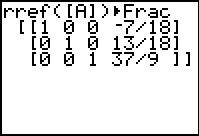
\includegraphics[width=2in]{./MatricesGraphics/RREF01.jpg} \hspace{.5in} & 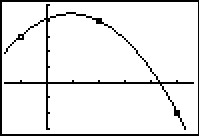
\includegraphics[width=2in]{./MatricesGraphics/QUADFIT01.jpg} \\
& The graph of $f(x) = -\frac{7}{18} x^2 + \frac{13}{18} x + \frac{37}{9}$ \\ & with the points $(-1,3)$, $(2,4)$ and $(5,-2)$ \\

\end{tabular}

\end{center}

\qed

\end{ex}

\newpage

\subsection{Exercises}

In Exercises \ref{rreffirst} - \ref{rreflast}, state whether the given matrix is in reduced row echelon form, row echelon form only or in neither of those forms.

\begin{multicols}{3} 
\begin{enumerate}


\item $\left[ \begin{array}{rr|r} 
1 & 0 & 3 \\ 
0 & 1 & 3  \\ 
\end{array} \right]$ \label{rreffirst}

\item $\left[ \begin{array}{rrr|r} 
3 & -1 & \hphantom{-}1 & 3 \\ 
2 & -4 & 3 & 16 \\ 
1 & -1 & 1 & 5  \\
\end{array} \right]$

\item $\left[ \begin{array}{rrr|r} 
1 & 1 & 4 & 3 \\ 
0 & 1 & 3 & 6 \\ 
0 & 0 & 0 & 1  \\
\end{array} \right]$

\setcounter{HW}{\value{enumi}}
\end{enumerate}
\end{multicols}

\begin{multicols}{3}
\begin{enumerate}
\setcounter{enumi}{\value{HW}}


\item $\left[ \begin{array}{rrr|r} 
1 & 0 & 0 & 0 \\ 
0 & 1 & 0 & 0 \\ 
0 & 0 & 0 & 1  \\
\end{array} \right]$

\item $\left[ \begin{array}{rrrr|r} 
1 & 0 & 4 & 3 & 0 \\ 
0 & 1 & 3 & 6 & 0 \\ 
0 & 0 & 0 & 0 & 0 
\end{array} \right]$

\item $\left[ \begin{array}{rrr|r} 
1 & 1 & 4 & 3 \\ 
0 & 1 & 3 & 6 \\
\end{array} \right]$ \label{rreflast}

\setcounter{HW}{\value{enumi}}
\end{enumerate}
\end{multicols}

In Exercises \ref{decodefirst} - \ref{decodelast}, the following matrices are in reduced row echelon form.  Determine the solution of the corresponding system of linear equations or state that the system is inconsistent.  


\begin{multicols}{3}
\begin{enumerate}
\setcounter{enumi}{\value{HW}}

\item $\left[ \begin{array}{rr|r} 
1 & 0 & -2 \\ 
0 & 1 & 7  \\ 
\end{array} \right]$  \label{decodefirst}

\item $\left[ \begin{array}{rrr|r} 
1 & 0 & 0 & -3 \\ 
0 & 1 & 0 & 20 \\ 
0 & 0 & 1 & 19  
\end{array} \right]$

\item $\left[ \begin{array}{rrrr|r} 
1 & 0 & 0 & 3 & 4 \\ 
0 & 1 & 0 & 6 & -6 \\ 
0 & 0 & 1 & 0 & 2 
\end{array} \right]$

\setcounter{HW}{\value{enumi}}
\end{enumerate}
\end{multicols}

\begin{multicols}{3}
\begin{enumerate}
\setcounter{enumi}{\value{HW}}

\item $\left[ \begin{array}{rrrr|r} 
1 & 0 & 0 & 3 & 0 \\ 
0 & 1 & 2 & 6 & 0 \\ 
0 & 0 & 0 & 0 & 1 
\end{array} \right]$

\item $\left[ \begin{array}{rrrr|r} 
1 & \hphantom{-}0 & -8 & 1 & 7 \\ 
0 & 1 & 4 & -3 & 2 \\ 
0 & 0 & 0 & 0 & 0 \\
0 & 0 & 0 & 0 & 0 
\end{array} \right]$

\item $\left[ \begin{array}{rrr|r} 
1 & \hphantom{-}0 & 9 & -3 \\ 
0 & 1 & -4 & 20 \\ 
0 & 0 & 0 & 0  
\end{array} \right]$ \label{decodelast}

\setcounter{HW}{\value{enumi}}
\end{enumerate}
\end{multicols}




In Exercises \ref{solveaugfirst} - \ref{solveauglast}, solve the following systems of linear equations using the techniques discussed in this section.  Compare and contrast these techniques with those you used to solve the systems in the Exercises in Section \ref{LinSystems}.

\begin{multicols}{2}
\begin{enumerate}
\setcounter{enumi}{\value{HW}}


\item $\left\{ \begin{array}{rcr} -5x + y & = & 17  \\ x + y & = & 5  \end{array} \right.$ \label{solveaugfirst}
\item $\left\{ \begin{array}{rcr} x + y + z & = & 3 \\ 2x - y + z & = & 0 \\ -3x + 5y + 7z & = & 7  \end{array} \right.$

\setcounter{HW}{\value{enumi}}
\end{enumerate}
\end{multicols}


\begin{multicols}{2}
\begin{enumerate}
\setcounter{enumi}{\value{HW}}


\item $\left\{ \begin{array}{rcr} 4x - y + z & = & 5 \\ 2y + 6z & = & 30 \\ x + z & = & 5  \end{array} \right.$

\item $\left\{ \begin{array}{rcr} x-2y+3z & = & 7 \\ -3x+y+2z & = & -5 \\ 2x+2y+z & = & 3  \end{array} \right.$

\setcounter{HW}{\value{enumi}}
\end{enumerate}
\end{multicols}


\begin{multicols}{2}
\begin{enumerate}
\setcounter{enumi}{\value{HW}}


\item $\left\{ \begin{array}{rcr} 3x-2y+z & = & -5 \\ x+3y-z & = & 12 \\ x+y+2z & = & 0  \end{array} \right.$
\item $\left\{ \begin{array}{rcr} 2x-y+z& = & -1 \\ 4x+3y+5z & = & 1 \\  5y+3z & = & 4 \end{array} \right.$

\setcounter{HW}{\value{enumi}}
\end{enumerate}
\end{multicols}


\begin{multicols}{2}
\begin{enumerate}
\setcounter{enumi}{\value{HW}}


\item $\left\{ \begin{array}{rcr} x-y+z & = & -4 \\ -3x+2y+4z & = & -5 \\ x-5y+2z & = & -18  \end{array} \right.$
\item $\left\{ \begin{array}{rcr} 2x-4y+z & = & -7 \\ x-2y+2z & = & -2 \\ -x+4y-2z & = & 3  \end{array} \right.$

\setcounter{HW}{\value{enumi}}
\end{enumerate}
\end{multicols}


\begin{multicols}{2}
\begin{enumerate}
\setcounter{enumi}{\value{HW}}


\item $\left\{ \begin{array}{rcr} 2x-y+z & = & 1 \\ 2x+2y-z & = & 1 \\ 3x+6y+4z & = & 9  \end{array} \right.$
\item $\left\{ \begin{array}{rcr} x-3y-4z & = & 3 \\ 3x+4y-z & = & 13 \\ 2x-19y-19z & = & 2  \end{array} \right.$

\setcounter{HW}{\value{enumi}}
\end{enumerate}
\end{multicols}


\begin{multicols}{2}
\begin{enumerate}
\setcounter{enumi}{\value{HW}}


\item $\left\{ \begin{array}{rcr} x+y+z & = & 4 \\ 2x-4y-z& = & -1 \\ x-y & = & 2 \end{array} \right.$
\item $\left\{ \begin{array}{rcr} x-y+z & = & 8 \\ 3x+3y-9z & = & -6 \\  7x-2y+5z & = & 39 \end{array} \right.$

\setcounter{HW}{\value{enumi}}
\end{enumerate}
\end{multicols}


\begin{multicols}{2}
\begin{enumerate}
\setcounter{enumi}{\value{HW}}


\item $\left\{ \begin{array}{rcr} 2x-3y+z & = & -1 \\ 4x-4y+4z & = & -13 \\ 6x-5y+7z & = & -25  \end{array} \right.$

\item  $\left\{ \begin{array}{rcr} x_{\mbox{\tiny$1$}} - x_{\mbox{\tiny$3$}} & = & -2 \\ 
2x_{\mbox{\tiny$2$}} - x_{\mbox{\tiny$4$}} & = & 0  \\  
x_{\mbox{\tiny$1$}} -  2x_{\mbox{\tiny$2$}} + x_{\mbox{\tiny$3$}} & = & 0 \\
-x_{\mbox{\tiny$3$}} + x_{\mbox{\tiny$4$}} & = & 1  \end{array} \right.$ \label{solveauglast}

\setcounter{HW}{\value{enumi}}
\end{enumerate}
\end{multicols}



\begin{enumerate}
\setcounter{enumi}{\value{HW}}

\item  It's time for another meal at our local buffet.  This time, 22 diners (5 of whom were children) feasted for $\$162.25$, before taxes.  If the kids buffet is $\$4.50$, the basic buffet is $\$7.50$, and the deluxe buffet (with crab legs) is $\$9.25$, find out how many diners chose the deluxe buffet. 

\item Carl wants to make a party mix consisting of almonds (which cost $\$7$ per pound), cashews (which cost $\$5$ per pound), and peanuts (which cost $\$2$ per pound.)  If he wants to make a $10$ pound mix with a budget of $\$35$, what are the possible combinations almonds, cashews, and peanuts?  (You may find it helpful to review Example \ref{lucasmixex} in Section \ref{LinSystems}.)


\item  Find the quadratic function passing through the points $(-2,1)$, $(1,4)$, $(3,-2)$

\item  At 9 PM, the temperature was $60^{\circ}$F; at midnight, the temperature was $50^{\circ}$F; and at 6 AM, the temperature was $70^{\circ}$F .  Use the technique in Example \ref{matrixcurvefitting} to fit a quadratic function to these data with the temperature, $T$, measured in degrees Fahrenheit, as the dependent variable, and the number of hours after 9 PM, $t$, measured in hours, as the independent variable. What was the coldest temperature of the night?  When did it occur? 

\item The price for admission into the Stitz-Zeager Sasquatch Museum and Research Station is \$15 for adults and \$8 for kids 13 years old and younger. When the Zahlenreich family visits the museum their bill is \$38 and when the Nullsatz family visits their bill is \$39.  One day both families went together and took an adult babysitter along to watch the kids and the total admission charge was \$92.  Later that summer, the adults from both families went without the kids and the bill was \$45.  Is that enough information to determine how many adults and children are in each family?  If not, state whether the resulting system is inconsistent or consistent dependent.  In the latter case, give at least two plausible solutions.  

\item Use the technique in Example \ref{matrixcurvefitting} to find the line between the points $(-3, 4)$ and $(6, 1)$. How does your answer compare to the slope-intercept form of the line in Equation \ref{slopeintercept}?

\item With the help of your classmates, find at least two different row echelon forms for the matrix \[\left[ \begin{array}{rr|r} 
1 & 2 & 3 \\ 
4 & 12 & 8  \\ 
\end{array} \right]\]

\end{enumerate}

\newpage

\subsection{Answers}

\begin{multicols}{2}
\begin{enumerate}

\item Reduced row echelon form
\item Neither

\setcounter{HW}{\value{enumi}}
\end{enumerate}
\end{multicols}


\begin{multicols}{2}
\begin{enumerate}
\setcounter{enumi}{\value{HW}}



\item Row echelon form only
\item Reduced row echelon form

\setcounter{HW}{\value{enumi}}
\end{enumerate}
\end{multicols}


\begin{multicols}{2}
\begin{enumerate}
\setcounter{enumi}{\value{HW}}

\item Reduced row echelon form
\item Row echelon form only

\setcounter{HW}{\value{enumi}}
\end{enumerate}
\end{multicols}

\begin{multicols}{2}
\begin{enumerate}
\setcounter{enumi}{\value{HW}}

\item $(-2, 7)$
\item $(-3, 20, 19)$

\setcounter{HW}{\value{enumi}}
\end{enumerate}
\end{multicols}


\begin{multicols}{2}
\begin{enumerate}
\setcounter{enumi}{\value{HW}}

\item $(-3t + 4, -6t - 6, 2, t)$ \\
for all real numbers $t$
\item Inconsistent


\setcounter{HW}{\value{enumi}}
\end{enumerate}
\end{multicols}


\begin{multicols}{2}
\begin{enumerate}
\setcounter{enumi}{\value{HW}}


\item $(8s - t + 7, -4s + 3t + 2, s, t)$ \\ for all real numbers $s$ and $t$
\item $(-9t - 3, 4t + 20, t)$ \\ for all real numbers $t$


\setcounter{HW}{\value{enumi}}
\end{enumerate}
\end{multicols}


\begin{multicols}{2}
\begin{enumerate}
\setcounter{enumi}{\value{HW}}

\item $(-2, 7)$
\item $(1, 2, 0)$

\setcounter{HW}{\value{enumi}}
\end{enumerate}
\end{multicols}


\begin{multicols}{2}
\begin{enumerate}
\setcounter{enumi}{\value{HW}}


\item $(-t + 5, -3t + 15, t)$\\
for all real numbers $t$
\item $(2,-1,1)$


\setcounter{HW}{\value{enumi}}
\end{enumerate}
\end{multicols}


\begin{multicols}{2}
\begin{enumerate}
\setcounter{enumi}{\value{HW}}

\item $(1,3,-2)$
\item Inconsistent


\setcounter{HW}{\value{enumi}}
\end{enumerate}
\end{multicols}


\begin{multicols}{2}
\begin{enumerate}
\setcounter{enumi}{\value{HW}}


\item $(1,3,-2)$
\item $\left(-3,\frac{1}{2},1\right)$

\setcounter{HW}{\value{enumi}}
\end{enumerate}
\end{multicols}


\begin{multicols}{2}
\begin{enumerate}
\setcounter{enumi}{\value{HW}}



\item  $\left(\frac{1}{3},\frac{2}{3},1\right)$
\item  $\left(\frac{19}{13} t + \frac{51}{13},-\frac{11}{13} t+\frac{4}{13},t\right)$\\
for all real numbers $t$

\setcounter{HW}{\value{enumi}}
\end{enumerate}
\end{multicols}


\begin{multicols}{2}
\begin{enumerate}
\setcounter{enumi}{\value{HW}}

\item Inconsistent
\item $\left(4,-3,1\right)$

\setcounter{HW}{\value{enumi}}
\end{enumerate}
\end{multicols}


\begin{multicols}{2}
\begin{enumerate}
\setcounter{enumi}{\value{HW}}


\item $\left(-2t - \frac{35}{4},-t - \frac{11}{2},t\right)$\\
for all real numbers $t$
\item $(1, 2, 3, 4)$

\setcounter{HW}{\value{enumi}}
\end{enumerate}
\end{multicols}

\begin{enumerate}
\setcounter{enumi}{\value{HW}}

\item  This time, 7 diners chose the deluxe buffet.

\item  If $t$ represents the amount (in pounds) of peanuts, then we need $1.5 t - 7.5$ pounds of almonds and $17.5 - 2.5t$ pounds of cashews.  Since we can't have a negative amount of nuts, $5 \leq t \leq 7$. 

\item  $f(x) = -\frac{4}{5} x^2+\frac{1}{5} x + \frac{23}{5}$

\item  $T(t) = \frac{20}{27} t^2 - \frac{50}{9} t + 60$.  Lowest temperature of the evening $\frac{595}{12} \approx 49.58^{\circ}$F at 12:45 AM.

\newpage

\item Let $x_{\mbox{\tiny$1$}}$ and $x_{\mbox{\tiny$2$}}$ be the numbers of adults and children, respectively, in the Zahlenreich family and let $x_{\mbox{\tiny$3$}}$ and $x_{\mbox{\tiny$4$}}$ be the numbers of adults and children, respectively, in the Nullsatz family.  The system of equations determined by the given information is 

$\left\{ \begin{array}{rcr} 15x_{\mbox{\tiny$1$}} + 8x_{\mbox{\tiny$2$}} & = & 38 \\ 
15x_{\mbox{\tiny$3$}} + 8x_{\mbox{\tiny$4$}} & = & 39  \\  
15x_{\mbox{\tiny$1$}} +  8x_{\mbox{\tiny$2$}} + 15x_{\mbox{\tiny$3$}} + 8x_{\mbox{\tiny$4$}} & = & 77 \\
15x_{\mbox{\tiny$1$}} + 15x_{\mbox{\tiny$3$}} & = & 45  \end{array} \right.$

We subtracted the cost of the babysitter in E3 so the constant is 77, not 92.  This system is consistent dependent and its solution is $\left(\frac{8}{15}t + \frac{2}{5}, -t + 4, -\frac{8}{15}t + \frac{13}{5}, t \right)$.  Our variables represent numbers of adults and children so they must be whole numbers.  Running through the values $t = 0, 1, 2, 3, 4$ yields only one solution where all four variables are whole numbers; $t = 3$ gives us $(2, 1, 1, 3)$.  Thus there are 2 adults and 1 child in the Zahlenreichs and 1 adult and 3 kids in the Nullsatzs.


\end{enumerate}

\closegraphsfile